\section{Options for Fake Point Source Injection Techniques}\label{sec:tech}

There are a variety of ways in which fake sources can be simulated and injected into the images. Some options are more suitable for transients (\S~\ref{ssec:tech_new}), and some for variable stars (\S~\ref{ssec:tech_pre}). The following is a precursory presentation of the options, some of which have been used in the science studies discussed in \S~\ref{sec:sci}. Typically, artificial sources -- positive or negative -- are added to the direct image {\it before} that image enters the difference imaging pipeline, so that the detection efficiency captures the end-to-end pipeline efficiency for detecting difference-image sources. (This is why fakes are not typically injected into the final difference image prior to source detection).

% % % % % % % % % % % % % % % % 
\subsection{Simulating New Fake Objects}\label{ssec:tech_new}

This applies to point sources that appear where there was no point source in the template image, such as transients like supernovae, variable stars that are undetectable in their quiescent state, and moving objects (assuming they're slow-moving enough to not appear as trailed sources, which is a different problem not included in this study). 

Artificial sources that represent new fake objects would be planted in and around galaxies in a way that samples the environments of known transients (and serves the use-cases of variable stars and moving objects projected on background galaxies), would adequately sample areas of open space where most moving objects, some variable stars, and high-$z$ transients with undetectable hosts will be found, and also in crowded fields where many variable stars will be discovered.

{\bf Model PSF ---} A 2D model for the PSF is added to the direct image in order to simulate a new point source. The shape of the PSF is derived from known trends with, e.g., the focal plane location or airmass (DCR), and the brighter/fatter effect.

{\bf Clone-Stamping ---} A nearby star is cut out and rescaled, and used as the simulated point source. One of the main drawbacks of using clone-stamping with LSST images is that incorporating the brighter/fatter effect into the simulation requires either that a star which is both nearby and of a similar brightness be used or that a model component added to the clone star to appropriately change the shape for the simulated brightness. Another drawback of clone-stamping is that very sparse/crowded fields might not have enough nearby/isolated point sources to use.

To decide between model PSFs and clone-stamping will require some testing in order to properly assess their performance and load on the computational resources. However, since knowing the PSF very accurately is something the LSST DMS will already be doing, it seems likely that the Model PSF option should be easier.

% % % % % % % % % % % % % % % % 
\subsection{Simulating Variability in Real Objects}\label{ssec:tech_pre}

This applies to point sources that appear in both the template and direct image, such as variable stars and AGN. In this case, artificial variability is added to an existing point source in the direct image. Extra steps would need to be taken to ensure any real, low-level variability does not affect the results.

{\bf Model PSF Variable Component ---} A 2D model for the PSF with the desired flux of the variable component of the source is added to the object's 2D profile. This might only be useful for probing small flux changes, as it would be difficult be consistent with the brighter/fatter effect.

{\bf Scaling-in-Place ---} Cutout the star, multiply its 2D profile by a scalar in order to make it brighter or fainter, and add it back to the image. This could be modified to account for the brighter/fatter effect by, e.g., convolving with a kernel that both applies the effect and the desired variability, instead of multiplying by a scalar.

\subsubsection{Planting in a Template Image}\label{ssec:tech_pre_temp}

Could there be situations in which, in order to simulate variability, adding a new point source to the template only, or to both the template and the direct image, is needed? For example, in crowded fields, the detection efficiency for variable components of stars that are faint in the template image might be difficult to accurately measure because faint stars are hard to detect and isolate in crowded fields. This a necessary step in applying either of the two above methods for injecting artificial variability in real objects. Thus, it might be necessary to simulate new faint stars in the template {\it and} the direct image, with some flux difference between them, in order to derive detection efficiencies that are not dominated by the brighter, more well-distinguished stars in a crowded field. This would add complexity to the issue and might further expand the scope of the proposed option to provide scientifically validated injected fakes. 

% % % % % % % % % % % % % % % % 
\section{Summary, Open Questions, and Suggested Future Work}\label{sec:future}

\begin{figure}
\begin{center}
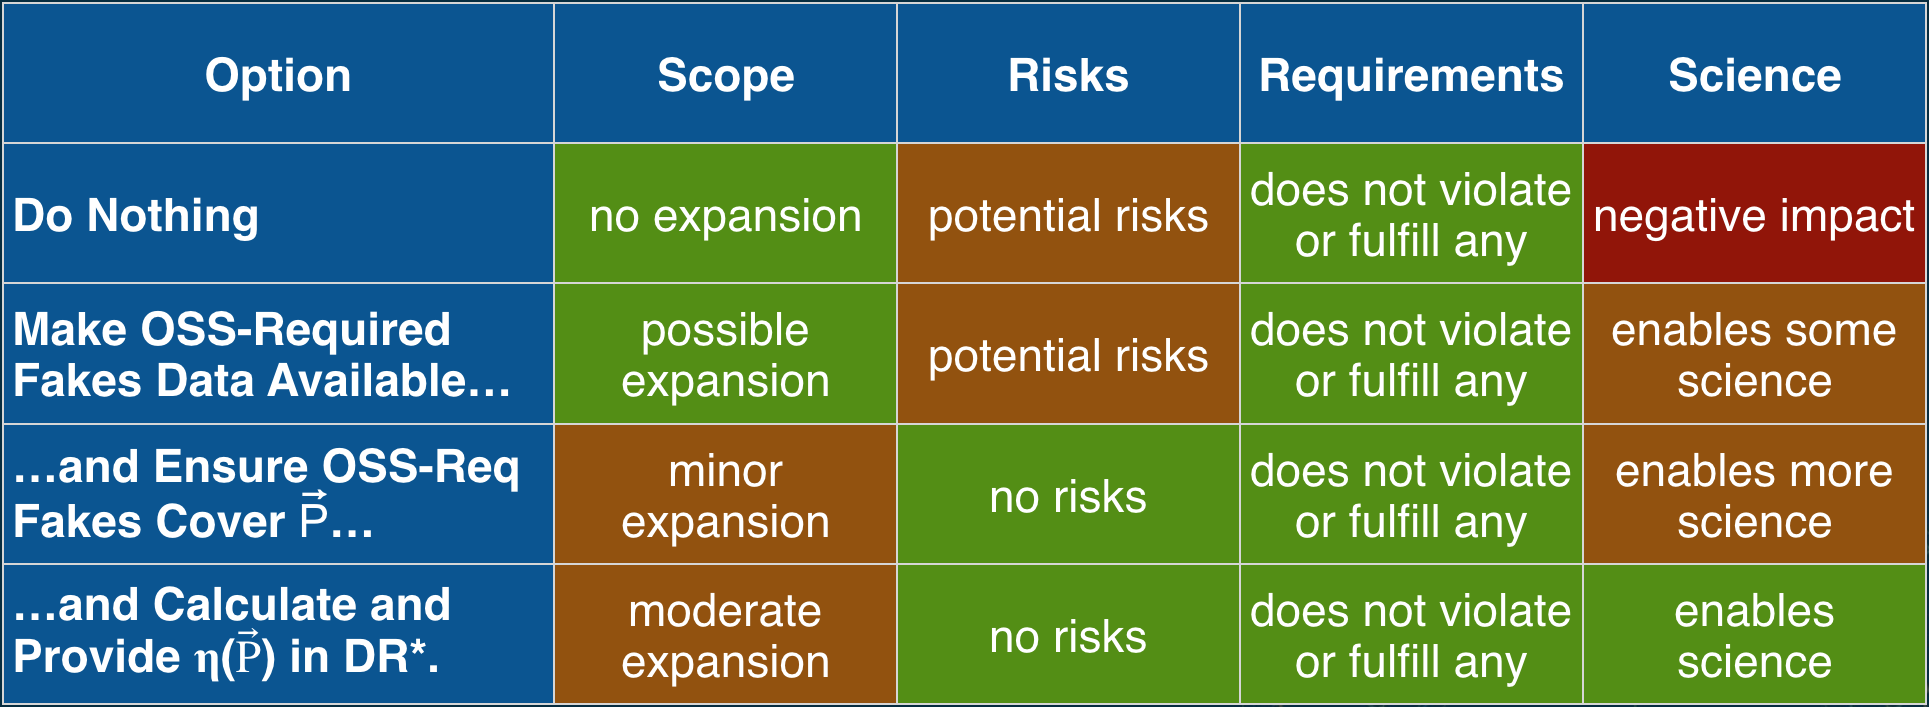
\includegraphics[width=15cm,trim={0cm 0cm 0cm 0cm}, clip]{figures/option_matrix.png}
\caption{A summary of the options with evaluated criteria, based on \S~\ref{sec:opts}. \label{fig:options}}
\end{center}
\end{figure}

This study is not yet finished and there remain some open questions to address, and further work is likely needed in order for an informed decision about the options proposed.

{\bf Open Questions for DM-SST:}\\
(1) Have DM's plans evolved away from what's in the documents (\S~\ref{sec:docs})? \\
(2) Does this work constitute a DMTN? It is not very technical -- yet. One option might be to take this to the TVS community for input and write a joint TVS-DM document, which incorporates the further study items below.

{\bf Further Study:}\\
 - establish the extent of the parameter space, $\vv{P}$\\
 - evaluate the accuracy needed for $\eta(\vv{P})$\\
 - does the mode of fake injection (\S~\ref{sec:opts}) matter for science?\\
 - will LSST's DIA be good enough to simply inject fakes into difference images?\\